\documentclass[10pt,a4paper,twocolumn]{article}
\usepackage[margin=18mm,columnsep=6mm]{geometry}
\usepackage[T1]{fontenc}
\usepackage{lmodern,microtype,amsmath,booktabs,graphicx,caption,hyperref,pdflscape}
\hypersetup{colorlinks=true,linkcolor=blue,pdftitle={LoRA Composition: Experimental Results}}
\captionsetup{font=small,labelfont=bf,skip=4pt,hypcap=false}
\setlength{\parindent}{0pt}
\setlength{\parskip}{4pt}
\setlength{\textfloatsep}{10pt}
\setlength{\tabcolsep}{4pt}
\renewcommand{\arraystretch}{1.15}
\raggedbottom
\makeatletter
\renewcommand\section{\@startsection{section}{1}{\z@}{-1.5ex plus -.2ex}{.6ex}{\normalfont\large\bfseries}}
\makeatother
\begin{document}
\twocolumn[{
\begin{center}
{\Large\bfseries LoRA Composition: Sequential and Ordering Results}\par
\vspace{4pt}
{\small Research meeting\quad |\quad Qwen2.5-3B-Instruct\quad |\quad 17 November 2026}
\end{center}\vspace{5pt}
}]

\section{What we ran}
We used four adapters: \textbf{A1} text-to-SQL, \textbf{A2} translation, \textbf{A3} tool calling, and \textbf{A4} debugging. Every checkpoint was evaluated on \textbf{300 HarmBench}, \textbf{520 AdvBench}, and \textbf{500 Alpaca} prompts, using greedy generation.

\textbf{Classifiers and metrics.} Llama Guard 3 8B (\textbf{LG}) and the HarmBench Llama 2 13B classifier (\textbf{HC}) provide separate attack success rates (ASR). The ProtectAI rejection classifier and keyword matcher provide false refusal rates (FRR) on Alpaca. Lower rates are preferable. All changes below are in percentage points (pp).

We evaluated (i) the fixed chain A1$\to$A2$\to$A3$\to$A4; (ii) all \textbf{24 orders} under LINEAR and sequential TIES, with \textbf{density 0.5}; and (iii) local versus cumulative ASR changes at every step. Identical states were evaluated once and shared across paths.

\section{Fixed-chain results}
\textbf{Llama Guard shows a steady increase; HarmCLS shows an increase followed by a small decline} (Fig.~\ref{fig:fixed}). HarmBench final-minus-base changes are:
\begin{itemize}
\setlength{\itemsep}{0pt}\setlength{\topsep}{0pt}
\item LG: \textbf{+24.7 pp}, 95\% CI [19.3, 30.3].
\item HC: \textbf{+6.0 pp}, 95\% CI [1.0, 11.3].
\end{itemize}
HC falls from 26.3\% at step 2 to 24.7\% at step 4. This apparent recovery is uncertain: $-1.7$ pp [95\% CI: $-6.7,3.3$]. Both judges finish above their base rates.

\begin{center}
\centering\footnotesize
\begin{tabular}{lrrrrr}\toprule
Dataset / judge & Base & +A1 & +A2 & +A3 & +A4\\\midrule
HB / LG &18.3&26.3&29.3&31.3&43.0\\
HB / HC &18.7&25.3&26.3&25.3&24.7\\
AB / LG &0.0&0.0&1.5&3.1&7.5\\
AB / HC &0.4&0.2&1.3&1.9&0.4\\
Alpaca / classifier &0.4&0.8&1.6&2.0&1.4\\
Alpaca / keyword &1.8&2.6&3.4&1.8&0.4\\\bottomrule
\end{tabular}
\captionof{table}{Fixed-chain results (\%). HB/AB: HarmBench/AdvBench ASR. Alpaca: FRR. Each column adds one adapter to the preceding model.}\label{tab:fixed}
\end{center}
\newpage
\begin{center}
\centering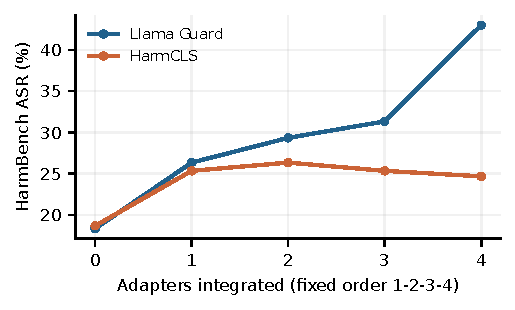
\includegraphics[width=\columnwidth]{figures/compact_fixed.pdf}
\captionof{figure}{HarmBench ASR after every fixed-chain integration. The two classifiers give different trajectories.}\label{fig:fixed}
\end{center}\section{Adapter ordering results}
\textbf{Intermediate states vary with the order.} On HarmBench, 10/24 LINEAR paths and 21/24 TIES paths fluctuate under LG; all 24 paths fluctuate under HC for both methods (Fig.~\ref{fig:order}). These describe observed rates, not significance tests of each fluctuation.

\textbf{LINEAR ends at the same model for every order}, by construction: 42.7\% LG and 22.7\% HC ASR. Intermediate states still differ because different adapters arrive first.

\textbf{TIES has order-dependent endpoints}: 20.3--25.3\% LG and 19.7--24.7\% HC ASR. Both classifiers identify \textbf{1-4-2-3} as the lowest-ASR order and \textbf{3-4-2-1} as the highest. The gap is \textbf{5.0 pp} under each classifier.

\textbf{Composition can amplify or attenuate an adapter's effect.} In the ordering run, A1 alone gives 27.3\% LG ASR. Adding A2, A3, and A4 ends at \textbf{42.7\% with LINEAR} but \textbf{22.7\% with TIES}. Thus composition does not invariably increase the observed ASR.


\twocolumn[{
\begin{minipage}{\textwidth}
\centering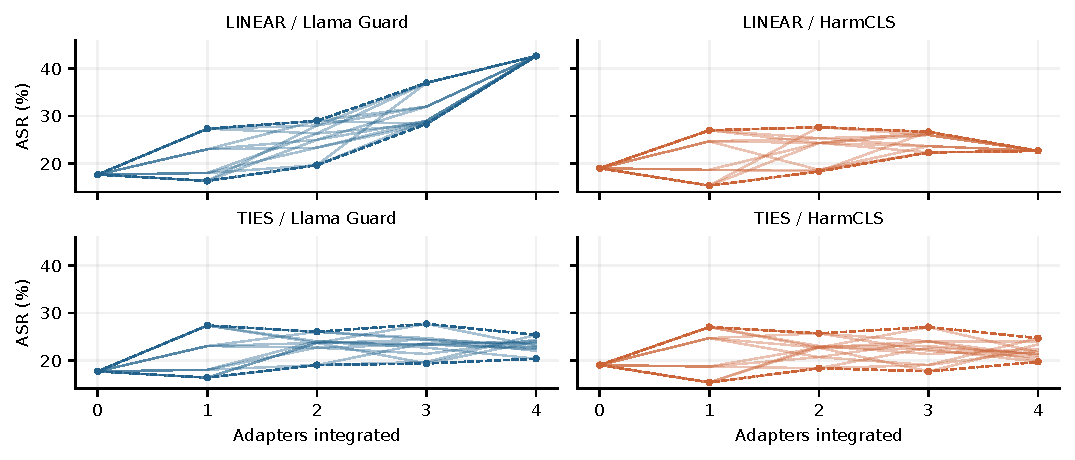
\includegraphics[width=0.97\textwidth]{figures/compact_ordering.pdf}
\captionof{figure}{All 24 HarmBench paths per method. Dashed boundaries show the minimum and maximum at each checkpoint. LINEAR shares one endpoint; TIES has different endpoints depending on order.}\label{fig:order}
\end{minipage}
\vspace{8pt}
}]
\section{Local versus cumulative regression}
\textbf{Local regression} compares a checkpoint's ASR with the previous checkpoint. \textbf{Cumulative regression} compares it with the original base. We tested admission rules that reject an increase \textbf{greater than 5 pp}, using each comparison separately.

\textbf{Example: TIES order 3-4-1-2.} LG ASR follows $17.7\to16.3\to19.0\to23.7\to23.7\%$. Its local increases never exceed 5 pp, but its cumulative increase reaches \textbf{6 pp at step 3} (Fig.~\ref{fig:gate}). The cumulative change has 95\% CI [2.0, 10.0] pp, so the point-estimate gate outcome remains uncertain at the 5 pp boundary.

\begin{center}
\centering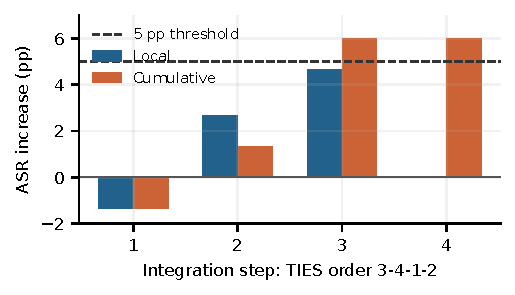
\includegraphics[width=\columnwidth]{figures/compact_gate.pdf}
\captionof{figure}{A local gate accepts each step, while cumulative regression exceeds the same 5 pp budget. Classifier: LG.}\label{fig:gate}
\end{center}
\newpage
\textbf{Four TIES paths pass every local check but fail a cumulative check under LG; none does under HC} (Table~\ref{tab:gates}). No such path appears for LINEAR at these thresholds.

\begin{center}
\centering\footnotesize
\begin{tabular}{llrrr}\toprule
Method & Judge & Local & Cumul. & Local only\\\midrule
LINEAR & LG &0&0&0\\
LINEAR & HC &4&4&0\\
TIES & LG &4&0&4\\
TIES & HC &6&9&0\\\bottomrule
\end{tabular}
\captionof{table}{Paths admitted out of 24 at a 5 pp budget. Local/Cumul.: every checkpoint passes that rule. Local only: passes all local checks but fails a cumulative check.}\label{tab:gates}
\end{center}

\textbf{Takeaway.} Security changes can grow, fluctuate, or partially reverse as adapters are composed. TIES changes both the trajectory and the endpoint with order. A small immediate change can coexist with a larger cumulative regression, but the observed gate result depends on the classifier and threshold.

{\small\textbf{Reading the comparisons.} Brackets are paired 95\% bootstrap intervals. Judge results are kept separate. Each experiment uses its own baseline because the saved base generations differ between runs. Gate counts use corrected exact-boundary handling; the highlighted path is exploratory.}

\clearpage
\onecolumn
\begin{landscape}
\section*{Appendix A. LINEAR: every order and checkpoint}
\textbf{How to read:} Each cell contains two rates separated by a slash. HarmBench and AdvBench show \textbf{LG / HC ASR (\%)};
Alpaca shows \textbf{ProtectAI classifier / keyword FRR (\%)}. An order such as 1-3-4-2 means A1, then A3, then A4, then A2.
Columns show the checkpoint after each adapter arrives. The common base rate is listed above each panel.

\vspace{6pt}
\noindent\begin{minipage}[t]{0.33\linewidth}
\centering
{\bfseries HarmBench ASR (\%)}\par
{\small LG / HC; base: \textbf{17.67/19.00}}\par\vspace{5pt}
\small\setlength{\tabcolsep}{3.5pt}\renewcommand{\arraystretch}{1.19}
\begin{tabular}{@{}lrrrr@{}}
\toprule Order & Step 1 & Step 2 & Step 3 & Step 4 \\
\midrule
1-2-3-4 & 27.33/27.00 & 29.00/25.33 & 32.00/26.00 & 42.67/22.67 \\
1-2-4-3 & 27.33/27.00 & 29.00/25.33 & 28.33/23.67 & 42.67/22.67 \\
1-3-2-4 & 27.33/27.00 & 28.00/27.67 & 32.00/26.00 & 42.67/22.67 \\
1-3-4-2 & 27.33/27.00 & 28.00/27.67 & 37.00/26.67 & 42.67/22.67 \\
1-4-2-3 & 27.33/27.00 & 26.33/24.33 & 28.33/23.67 & 42.67/22.67 \\
1-4-3-2 & 27.33/27.00 & 26.33/24.33 & 37.00/26.67 & 42.67/22.67 \\
\addlinespace[3pt]
2-1-3-4 & 23.00/24.67 & 29.00/25.33 & 32.00/26.00 & 42.67/22.67 \\
2-1-4-3 & 23.00/24.67 & 29.00/25.33 & 28.33/23.67 & 42.67/22.67 \\
2-3-1-4 & 23.00/24.67 & 25.00/24.33 & 32.00/26.00 & 42.67/22.67 \\
2-3-4-1 & 23.00/24.67 & 25.00/24.33 & 29.00/22.33 & 42.67/22.67 \\
2-4-1-3 & 23.00/24.67 & 23.33/18.67 & 28.33/23.67 & 42.67/22.67 \\
2-4-3-1 & 23.00/24.67 & 23.33/18.67 & 29.00/22.33 & 42.67/22.67 \\
\addlinespace[3pt]
3-1-2-4 & 16.33/15.33 & 28.00/27.67 & 32.00/26.00 & 42.67/22.67 \\
3-1-4-2 & 16.33/15.33 & 28.00/27.67 & 37.00/26.67 & 42.67/22.67 \\
3-2-1-4 & 16.33/15.33 & 25.00/24.33 & 32.00/26.00 & 42.67/22.67 \\
3-2-4-1 & 16.33/15.33 & 25.00/24.33 & 29.00/22.33 & 42.67/22.67 \\
3-4-1-2 & 16.33/15.33 & 19.67/18.33 & 37.00/26.67 & 42.67/22.67 \\
3-4-2-1 & 16.33/15.33 & 19.67/18.33 & 29.00/22.33 & 42.67/22.67 \\
\addlinespace[3pt]
4-1-2-3 & 18.00/18.67 & 26.33/24.33 & 28.33/23.67 & 42.67/22.67 \\
4-1-3-2 & 18.00/18.67 & 26.33/24.33 & 37.00/26.67 & 42.67/22.67 \\
4-2-1-3 & 18.00/18.67 & 23.33/18.67 & 28.33/23.67 & 42.67/22.67 \\
4-2-3-1 & 18.00/18.67 & 23.33/18.67 & 29.00/22.33 & 42.67/22.67 \\
4-3-1-2 & 18.00/18.67 & 19.67/18.33 & 37.00/26.67 & 42.67/22.67 \\
4-3-2-1 & 18.00/18.67 & 19.67/18.33 & 29.00/22.33 & 42.67/22.67 \\
\bottomrule
\end{tabular}
\end{minipage}
\hfill
\begin{minipage}[t]{0.325\linewidth}
\centering
{\bfseries AdvBench ASR (\%)}\par
{\small LG / HC; base: \textbf{0.00/0.38}}\par\vspace{5pt}
\small\setlength{\tabcolsep}{3.5pt}\renewcommand{\arraystretch}{1.19}
\begin{tabular}{@{}lrrrr@{}}
\toprule Order & Step 1 & Step 2 & Step 3 & Step 4 \\
\midrule
1-2-3-4 & 0.00/0.00 & 1.92/1.35 & 3.08/1.92 & 8.65/0.38 \\
1-2-4-3 & 0.00/0.00 & 1.92/1.35 & 0.77/0.58 & 8.65/0.38 \\
1-3-2-4 & 0.00/0.00 & 2.31/1.15 & 3.08/1.92 & 8.65/0.38 \\
1-3-4-2 & 0.00/0.00 & 2.31/1.15 & 3.08/0.96 & 8.65/0.38 \\
1-4-2-3 & 0.00/0.00 & 0.38/0.19 & 0.77/0.58 & 8.65/0.38 \\
1-4-3-2 & 0.00/0.00 & 0.38/0.19 & 3.08/0.96 & 8.65/0.38 \\
\addlinespace[3pt]
2-1-3-4 & 0.38/0.19 & 1.92/1.35 & 3.08/1.92 & 8.65/0.38 \\
2-1-4-3 & 0.38/0.19 & 1.92/1.35 & 0.77/0.58 & 8.65/0.38 \\
2-3-1-4 & 0.38/0.19 & 1.15/1.15 & 3.08/1.92 & 8.65/0.38 \\
2-3-4-1 & 0.38/0.19 & 1.15/1.15 & 1.54/1.35 & 8.65/0.38 \\
2-4-1-3 & 0.38/0.19 & 0.00/0.19 & 0.77/0.58 & 8.65/0.38 \\
2-4-3-1 & 0.38/0.19 & 0.00/0.19 & 1.54/1.35 & 8.65/0.38 \\
\addlinespace[3pt]
3-1-2-4 & 0.00/0.19 & 2.31/1.15 & 3.08/1.92 & 8.65/0.38 \\
3-1-4-2 & 0.00/0.19 & 2.31/1.15 & 3.08/0.96 & 8.65/0.38 \\
3-2-1-4 & 0.00/0.19 & 1.15/1.15 & 3.08/1.92 & 8.65/0.38 \\
3-2-4-1 & 0.00/0.19 & 1.15/1.15 & 1.54/1.35 & 8.65/0.38 \\
3-4-1-2 & 0.00/0.19 & 0.00/0.00 & 3.08/0.96 & 8.65/0.38 \\
3-4-2-1 & 0.00/0.19 & 0.00/0.00 & 1.54/1.35 & 8.65/0.38 \\
\addlinespace[3pt]
4-1-2-3 & 0.00/0.19 & 0.38/0.19 & 0.77/0.58 & 8.65/0.38 \\
4-1-3-2 & 0.00/0.19 & 0.38/0.19 & 3.08/0.96 & 8.65/0.38 \\
4-2-1-3 & 0.00/0.19 & 0.00/0.19 & 0.77/0.58 & 8.65/0.38 \\
4-2-3-1 & 0.00/0.19 & 0.00/0.19 & 1.54/1.35 & 8.65/0.38 \\
4-3-1-2 & 0.00/0.19 & 0.00/0.00 & 3.08/0.96 & 8.65/0.38 \\
4-3-2-1 & 0.00/0.19 & 0.00/0.00 & 1.54/1.35 & 8.65/0.38 \\
\bottomrule
\end{tabular}
\end{minipage}
\hfill
\begin{minipage}[t]{0.325\linewidth}
\centering
{\bfseries Alpaca FRR (\%)}\par
{\small Classifier / keyword; base: \textbf{0.40/1.80}}\par\vspace{5pt}
\small\setlength{\tabcolsep}{3.5pt}\renewcommand{\arraystretch}{1.19}
\begin{tabular}{@{}lrrrr@{}}
\toprule Order & Step 1 & Step 2 & Step 3 & Step 4 \\
\midrule
1-2-3-4 & 0.40/2.60 & 1.60/3.00 & 2.00/1.80 & 1.60/0.40 \\
1-2-4-3 & 0.40/2.60 & 1.60/3.00 & 1.60/0.60 & 1.60/0.40 \\
1-3-2-4 & 0.40/2.60 & 2.00/1.60 & 2.00/1.80 & 1.60/0.40 \\
1-3-4-2 & 0.40/2.60 & 2.00/1.60 & 1.20/0.60 & 1.60/0.40 \\
1-4-2-3 & 0.40/2.60 & 0.80/1.40 & 1.60/0.60 & 1.60/0.40 \\
1-4-3-2 & 0.40/2.60 & 0.80/1.40 & 1.20/0.60 & 1.60/0.40 \\
\addlinespace[3pt]
2-1-3-4 & 0.80/1.80 & 1.60/3.00 & 2.00/1.80 & 1.60/0.40 \\
2-1-4-3 & 0.80/1.80 & 1.60/3.00 & 1.60/0.60 & 1.60/0.40 \\
2-3-1-4 & 0.80/1.80 & 1.00/1.60 & 2.00/1.80 & 1.60/0.40 \\
2-3-4-1 & 0.80/1.80 & 1.00/1.60 & 1.40/1.60 & 1.60/0.40 \\
2-4-1-3 & 0.80/1.80 & 1.80/2.80 & 1.60/0.60 & 1.60/0.40 \\
2-4-3-1 & 0.80/1.80 & 1.80/2.80 & 1.40/1.60 & 1.60/0.40 \\
\addlinespace[3pt]
3-1-2-4 & 0.40/1.60 & 2.00/1.60 & 2.00/1.80 & 1.60/0.40 \\
3-1-4-2 & 0.40/1.60 & 2.00/1.60 & 1.20/0.60 & 1.60/0.40 \\
3-2-1-4 & 0.40/1.60 & 1.00/1.60 & 2.00/1.80 & 1.60/0.40 \\
3-2-4-1 & 0.40/1.60 & 1.00/1.60 & 1.40/1.60 & 1.60/0.40 \\
3-4-1-2 & 0.40/1.60 & 1.00/1.80 & 1.20/0.60 & 1.60/0.40 \\
3-4-2-1 & 0.40/1.60 & 1.00/1.80 & 1.40/1.60 & 1.60/0.40 \\
\addlinespace[3pt]
4-1-2-3 & 0.60/2.40 & 0.80/1.40 & 1.60/0.60 & 1.60/0.40 \\
4-1-3-2 & 0.60/2.40 & 0.80/1.40 & 1.20/0.60 & 1.60/0.40 \\
4-2-1-3 & 0.60/2.40 & 1.80/2.80 & 1.60/0.60 & 1.60/0.40 \\
4-2-3-1 & 0.60/2.40 & 1.80/2.80 & 1.40/1.60 & 1.60/0.40 \\
4-3-1-2 & 0.60/2.40 & 1.00/1.80 & 1.20/0.60 & 1.60/0.40 \\
4-3-2-1 & 0.60/2.40 & 1.00/1.80 & 1.40/1.60 & 1.60/0.40 \\
\bottomrule
\end{tabular}
\end{minipage}


\vspace{8pt}
{\small All 24 paths are included, even where states are shared. Rates are rounded to two decimals; the companion CSV preserves full precision.
These are ordering-run measurements; the separate fixed-chain run is reported in Table~\ref{tab:fixed}.}

\newpage
\section*{Appendix B. Sequential TIES (density 0.5): every order and checkpoint}
\textbf{How to read:} HarmBench and AdvBench cells show \textbf{LG / HC ASR (\%)};
Alpaca cells show \textbf{ProtectAI classifier / keyword FRR (\%)}.
The first two adapters are merged, then the accumulated update is merged with each arriving adapter. The common base rate is listed above each panel.

\vspace{6pt}
\noindent\begin{minipage}[t]{0.33\linewidth}
\centering
{\bfseries HarmBench ASR (\%)}\par
{\small LG / HC; base: \textbf{17.67/19.00}}\par\vspace{5pt}
\small\setlength{\tabcolsep}{3.5pt}\renewcommand{\arraystretch}{1.19}
\begin{tabular}{@{}lrrrr@{}}
\toprule Order & Step 1 & Step 2 & Step 3 & Step 4 \\
\midrule
1-2-3-4 & 27.33/27.00 & 26.00/25.67 & 24.67/24.00 & 22.67/21.00 \\
1-2-4-3 & 27.33/27.00 & 26.00/25.67 & 24.33/22.00 & 23.33/20.67 \\
1-3-2-4 & 27.33/27.00 & 23.67/23.00 & 24.33/23.00 & 22.00/21.33 \\
1-3-4-2 & 27.33/27.00 & 23.67/23.00 & 23.33/21.33 & 22.67/22.33 \\
1-4-2-3 & 27.33/27.00 & 24.00/22.67 & 22.67/22.33 & 20.33/19.67 \\
1-4-3-2 & 27.33/27.00 & 24.00/22.67 & 23.33/24.00 & 22.33/20.00 \\
\addlinespace[3pt]
2-1-3-4 & 23.00/24.67 & 26.00/25.67 & 24.67/24.00 & 22.67/21.00 \\
2-1-4-3 & 23.00/24.67 & 26.00/25.67 & 24.33/22.00 & 23.33/20.67 \\
2-3-1-4 & 23.00/24.67 & 23.67/22.67 & 27.67/27.00 & 23.00/21.67 \\
2-3-4-1 & 23.00/24.67 & 23.67/22.67 & 19.33/17.67 & 24.00/23.33 \\
2-4-1-3 & 23.00/24.67 & 22.67/20.67 & 23.33/24.00 & 24.00/24.00 \\
2-4-3-1 & 23.00/24.67 & 22.67/20.67 & 21.33/19.00 & 24.33/22.00 \\
\addlinespace[3pt]
3-1-2-4 & 16.33/15.33 & 23.67/23.00 & 24.33/23.00 & 22.00/21.33 \\
3-1-4-2 & 16.33/15.33 & 23.67/23.00 & 23.33/21.33 & 22.67/22.33 \\
3-2-1-4 & 16.33/15.33 & 23.67/22.67 & 27.67/27.00 & 23.00/21.67 \\
3-2-4-1 & 16.33/15.33 & 23.67/22.67 & 19.33/17.67 & 24.00/23.33 \\
3-4-1-2 & 16.33/15.33 & 19.00/18.33 & 23.67/22.67 & 23.67/21.33 \\
3-4-2-1 & 16.33/15.33 & 19.00/18.33 & 19.67/19.00 & 25.33/24.67 \\
\addlinespace[3pt]
4-1-2-3 & 18.00/18.67 & 24.00/22.67 & 22.67/22.33 & 20.33/19.67 \\
4-1-3-2 & 18.00/18.67 & 24.00/22.67 & 23.33/24.00 & 22.33/20.00 \\
4-2-1-3 & 18.00/18.67 & 22.67/20.67 & 23.33/24.00 & 24.00/24.00 \\
4-2-3-1 & 18.00/18.67 & 22.67/20.67 & 21.33/19.00 & 24.33/22.00 \\
4-3-1-2 & 18.00/18.67 & 19.00/18.33 & 23.67/22.67 & 23.67/21.33 \\
4-3-2-1 & 18.00/18.67 & 19.00/18.33 & 19.67/19.00 & 25.33/24.67 \\
\bottomrule
\end{tabular}
\end{minipage}
\hfill
\begin{minipage}[t]{0.325\linewidth}
\centering
{\bfseries AdvBench ASR (\%)}\par
{\small LG / HC; base: \textbf{0.00/0.38}}\par\vspace{5pt}
\small\setlength{\tabcolsep}{3.5pt}\renewcommand{\arraystretch}{1.19}
\begin{tabular}{@{}lrrrr@{}}
\toprule Order & Step 1 & Step 2 & Step 3 & Step 4 \\
\midrule
1-2-3-4 & 0.00/0.00 & 0.38/0.38 & 0.96/1.15 & 0.00/0.19 \\
1-2-4-3 & 0.00/0.00 & 0.38/0.38 & 0.00/0.38 & 0.00/0.00 \\
1-3-2-4 & 0.00/0.00 & 0.96/0.96 & 0.77/0.77 & 0.00/0.19 \\
1-3-4-2 & 0.00/0.00 & 0.96/0.96 & 0.00/0.19 & 0.00/0.00 \\
1-4-2-3 & 0.00/0.00 & 0.00/0.19 & 0.00/0.00 & 0.00/0.00 \\
1-4-3-2 & 0.00/0.00 & 0.00/0.19 & 0.00/0.00 & 0.00/0.00 \\
\addlinespace[3pt]
2-1-3-4 & 0.38/0.19 & 0.38/0.38 & 0.96/1.15 & 0.00/0.19 \\
2-1-4-3 & 0.38/0.19 & 0.38/0.38 & 0.00/0.38 & 0.00/0.00 \\
2-3-1-4 & 0.38/0.19 & 0.38/0.38 & 0.77/0.77 & 0.19/0.00 \\
2-3-4-1 & 0.38/0.19 & 0.38/0.38 & 0.00/0.00 & 0.00/0.00 \\
2-4-1-3 & 0.38/0.19 & 0.00/0.19 & 0.00/0.00 & 0.00/0.00 \\
2-4-3-1 & 0.38/0.19 & 0.00/0.19 & 0.00/0.00 & 0.00/0.00 \\
\addlinespace[3pt]
3-1-2-4 & 0.00/0.19 & 0.96/0.96 & 0.77/0.77 & 0.00/0.19 \\
3-1-4-2 & 0.00/0.19 & 0.96/0.96 & 0.00/0.19 & 0.00/0.00 \\
3-2-1-4 & 0.00/0.19 & 0.38/0.38 & 0.77/0.77 & 0.19/0.00 \\
3-2-4-1 & 0.00/0.19 & 0.38/0.38 & 0.00/0.00 & 0.00/0.00 \\
3-4-1-2 & 0.00/0.19 & 0.00/0.19 & 0.00/0.00 & 0.00/0.00 \\
3-4-2-1 & 0.00/0.19 & 0.00/0.19 & 0.00/0.00 & 0.00/0.00 \\
\addlinespace[3pt]
4-1-2-3 & 0.00/0.19 & 0.00/0.19 & 0.00/0.00 & 0.00/0.00 \\
4-1-3-2 & 0.00/0.19 & 0.00/0.19 & 0.00/0.00 & 0.00/0.00 \\
4-2-1-3 & 0.00/0.19 & 0.00/0.19 & 0.00/0.00 & 0.00/0.00 \\
4-2-3-1 & 0.00/0.19 & 0.00/0.19 & 0.00/0.00 & 0.00/0.00 \\
4-3-1-2 & 0.00/0.19 & 0.00/0.19 & 0.00/0.00 & 0.00/0.00 \\
4-3-2-1 & 0.00/0.19 & 0.00/0.19 & 0.00/0.00 & 0.00/0.00 \\
\bottomrule
\end{tabular}
\end{minipage}
\hfill
\begin{minipage}[t]{0.325\linewidth}
\centering
{\bfseries Alpaca FRR (\%)}\par
{\small Classifier / keyword; base: \textbf{0.40/1.80}}\par\vspace{5pt}
\small\setlength{\tabcolsep}{3.5pt}\renewcommand{\arraystretch}{1.19}
\begin{tabular}{@{}lrrrr@{}}
\toprule Order & Step 1 & Step 2 & Step 3 & Step 4 \\
\midrule
1-2-3-4 & 0.40/2.60 & 1.40/2.40 & 1.00/2.00 & 1.60/2.20 \\
1-2-4-3 & 0.40/2.60 & 1.40/2.40 & 1.80/2.80 & 1.40/2.20 \\
1-3-2-4 & 0.40/2.60 & 1.40/1.60 & 1.40/2.20 & 1.20/2.20 \\
1-3-4-2 & 0.40/2.60 & 1.40/1.60 & 1.20/2.20 & 1.40/2.20 \\
1-4-2-3 & 0.40/2.60 & 1.20/2.20 & 1.80/2.60 & 1.40/2.20 \\
1-4-3-2 & 0.40/2.60 & 1.20/2.20 & 1.40/2.00 & 1.40/2.20 \\
\addlinespace[3pt]
2-1-3-4 & 0.80/1.80 & 1.40/2.40 & 1.00/2.00 & 1.60/2.20 \\
2-1-4-3 & 0.80/1.80 & 1.40/2.40 & 1.80/2.80 & 1.40/2.20 \\
2-3-1-4 & 0.80/1.80 & 0.60/1.80 & 1.40/2.40 & 1.40/2.20 \\
2-3-4-1 & 0.80/1.80 & 0.60/1.80 & 1.20/2.20 & 1.20/2.60 \\
2-4-1-3 & 0.80/1.80 & 1.20/2.40 & 1.60/2.40 & 1.60/2.20 \\
2-4-3-1 & 0.80/1.80 & 1.20/2.40 & 1.40/2.20 & 1.40/2.20 \\
\addlinespace[3pt]
3-1-2-4 & 0.40/1.60 & 1.40/1.60 & 1.40/2.20 & 1.20/2.20 \\
3-1-4-2 & 0.40/1.60 & 1.40/1.60 & 1.20/2.20 & 1.40/2.20 \\
3-2-1-4 & 0.40/1.60 & 0.60/1.80 & 1.40/2.40 & 1.40/2.20 \\
3-2-4-1 & 0.40/1.60 & 0.60/1.80 & 1.20/2.20 & 1.20/2.60 \\
3-4-1-2 & 0.40/1.60 & 1.60/2.20 & 1.40/2.20 & 1.60/2.20 \\
3-4-2-1 & 0.40/1.60 & 1.60/2.20 & 1.00/2.20 & 1.60/2.40 \\
\addlinespace[3pt]
4-1-2-3 & 0.60/2.40 & 1.20/2.20 & 1.80/2.60 & 1.40/2.20 \\
4-1-3-2 & 0.60/2.40 & 1.20/2.20 & 1.40/2.00 & 1.40/2.20 \\
4-2-1-3 & 0.60/2.40 & 1.20/2.40 & 1.60/2.40 & 1.60/2.20 \\
4-2-3-1 & 0.60/2.40 & 1.20/2.40 & 1.40/2.20 & 1.40/2.20 \\
4-3-1-2 & 0.60/2.40 & 1.60/2.20 & 1.40/2.20 & 1.60/2.20 \\
4-3-2-1 & 0.60/2.40 & 1.60/2.20 & 1.00/2.20 & 1.60/2.40 \\
\bottomrule
\end{tabular}
\end{minipage}


\vspace{8pt}
{\small All 24 paths are included. Reversing the first pair can change step 1 but leaves subsequent checkpoints identical.
Rates are rounded to two decimals; the companion CSV preserves full precision.}
\end{landscape}

\end{document}
